\documentclass[pdftex,12pt,a4paper]{report}
\usepackage{dbstmpl}

% Hier die eigenen Daten eintragen
\global\arbeit{Bachelor Thesis}
\global\titel{Optical Character Recognition for Labels Using Deep Learning}
\global\bearbeiter{Johannes Reichle}
\global\matrikel{04797218}
\global\betreuer{Prof.\ Dr.\ Rainer Schmidt}
\global\aufgabensteller{Random Ltd.}
\global\abgabetermin{XX.XX.2022}
\global\ort{Munich}
\global\fach{Information Systems and Management}

\begin{document}

\deckblatt
\erklaerung

\begin{abstract}
    Here abstract for \the\arbeit.
\end{abstract}


\tableofcontents
\listoffigures
% delete group thing to have tables on new page
\begingroup
    \let\clearpage\relax
    \listoftables
\endgroup

\chapter*{Abbreviations}
\addcontentsline{toc}{chapter}{Abbreviations}
\printacronyms[heading=none]

\chapter{Introduction}\label{ch:intro}
\section{Motivation}
\ac{OCR} is the concept of extracting typed, handwritten or printed text
from an image.
Techniques for this concept have improved a lot due to the advances in the field of
\ac{DL}~\citep{zhao_improving_2020}.
When compared to traditional methods \ac{DL} improves automation, effectiveness and
generalization~\citep{chen_text_2021}.
\ac{DL} is a technology based on \acp{NN} where data is processed
in multiple layers to extract complex features to solve a given problem~\citep{shrestha_review_2019}.
\ac{DL} has only caught on in the recent years as the big computational cost has been met
by improvement in computer hardware as well as automatic feature
learning~\citep{ponti_everything_2017, chen_text_2021}.
Finding the right solution in the space of \ac{DL} and applying these new capabilities to
the use case of extracting information of labels is the focus of this thesis.
This is an interesting task as performance of \ac{OCR} systems in complex scenes is still
challenging~\citep{zhao_improving_2020}.
Such scenes entail natural scenes captured by a camera.
\ac{OCR} in these conditions is also known as \ac{STR}~\citep{chen_text_2021}.
Factors such as complex backgrounds, noise, perspective and variability in fonts, colors and sizes,
of scene texts complicate the process~\citep{hu_gtc_2020,chen_text_2021}.
Therefore, it is critical to specify possible factors for the underlying problem and to find
criteria for evaluating feasibility.

% FIXME: adjust for pipeline instead of model
\section{Problem description}\label{se:problem}
The basic problem of this thesis is finding a viable solution for the extraction of textual
information from images with equipment labels.
However, it is difficult to assess how well an approach performs before it has been implemented and
tested on the specific problem or dataset~\citep{arpteg_software_2018}.
Therefore, it is useful to propose several approaches that might solve the problem from
different angles and different properties.

The problem has to first be analyzed in depth in order to find viable approaches for the solution.
This includes defining requirements such as detecting alpha-numeric strings or suitability despite
inadequate image conditions~\citep{ghosh_visual_2017, hu_gtc_2020}.
These requirements define properties that an approach must have in order to be classified as viable.
Thus the reasearch and subsequent discussion of techniques from end-to-end \ac{OCR} to dividing the
process into text detection and text recognition is centered around the requirements which are
given by the problem.

Subsequent aspects such as implementation, training, deployment and maintenance of a solution in a
production environment shall not be performed within the scope of this thesis.
However, because these aspects may vary depending on the approach, it is important to consider them when
discussing the viability for solving the problem.

% FIXME: add following
only model selection activity~\citep{ashmore_assuring_2021}
set into context to MLC lifecycle: Data Management, Model Learning (Model Selection, Training,
Transfer Learning, Hyperparameter Selection), Model Verificatoin

\section{Methodology}\label{se:methodology}
The methodology of this thesis can be described as a literature review.
As such, the research question guiding the process is most crucial: Which state of the art \ac{DL}
approaches for \ac{OCR} are viable for the use case of extracting textual label data from
images.
The following section describes how relevant literature is identified, analyzed and synthesised.

\section{Expected results}
% FIXME: kürzen
% FIXME: weg von literature review -> problem with criteria, analysing and summarizing research,
%               find viable approaches and compare properties for 5
In addition to a deeper understanding of the problem and its detailed definition, the literature
review lays the foundation for finding the right approach for the extraction of textual
information from images with equipment labels through literature review.
In the subsequent analysis different approaches are highlighted for their theoretical fit as a solution.

In the following section the structure of this thesis is listed and each chapter's expected
result is detailed along with its benefits for the overall objective of producing an overview of
state of the art \ac{OCR} relevant for the problem described in Section~\ref{se:problem}.
comprehension of the following chapters is gathered.
% FIXME: grammar above
This includes general principles of \ac{DL} and by extension \ac{ML} but also of \ac{OCR}.\@
In Chapter~\ref{ch:problem} the problem from Section~\ref{se:problem} is addressed in more detail.
The result shall be a firm understanding of functional and non-functional requirements both on the
technical and the business process side.
% FIXME: add exclusion criteria
These requirements are the point of focus for the further examination of \ac{OCR} techniques.
After laying the foundation, in Chapter~\ref{ch:research} current research in regards to the
identified requirements is examined.
The resulting overview can be viewed as a basis for a decision when it comes implementing a practical
solution.
Therefore it enables the discussion in Chapter~\ref{ch:discussion}.
Here not only the results and the availability of a solution but also the methodology of this work
are assessed critically.
The conclusion is a summary of the results compared to the expected results detailed in this chapter
as well as an outlook for further research into the topic.

\chapter{Problem analysis}\label{ch:problem}
This chapter entails an analysis of the problem which is the research question's foundation.
It is crucial, as the quality of requirements ultimately determines the quality of the literature review.

%\section{Requirements}
For traditional software projects requirements engineering classifies requirements into
two categories~\cite{zowghi_requirements_2014}.
\Acp{FR} specify functionality that users can experience~\cite{noauthor_ieee_1998}.
Other requirements that are relevant to the project in a way that shapes the target system,
defines the development process and manages the development project are refered to as
\acp{NFR}~\cite{kotonya_requirements_1998,chung_non-functional_2009}.
For \ac{ML} and thus \ac{DL} projects, data directly influences the performance of the solution.
This results in the need to specify \acp{DR} for data that is used
in conjunction with the \ac{DL} system~\cite{vogelsang_requirements_2019}.

% FIXME: add that requirements where not gathered according to normal processes (like stakeholder
analysis\ldots

% FIXME: only model requirements, maybe get rid of data requirements entirely
% FIXME: find exlusion criteria
% alphanumeric strings, preserve saving and strucure with coordinates,
% computationally efficient (how to define cutof)
% --> all FR without performance metric?

% functional requirements
The basic functionality can be described as extraction of textual data from images.
The relevant text information is framed by a label.
The label contains printed text which can be structured and spaced differently from label to
label (see figure~\ref{fig:examples}).
\begin{figure}
    \centering
    \subfigure[Positive example\label{fig:good-example}]{\includegraphics[width=0.48\textwidth]{img/Image-Example-Positive.jpg}}
    \subfigure[Negative example\label{fig:bad-example}]{\includegraphics[width=0.48\textwidth]{img/Image-Example-Negative.jpg}}
    \caption{Examples for label images\label{fig:examples}}
\end{figure}
The text carries semantic information which can be important for later processing in the scope of
a business process.
The goal is to extract the text and preserve semantics from structure and space.
This means text and the respective coordinates, height, width and a possible rotation angle must
be output as the result~\cite{yang_learning_2021}.
Those values can then be transformed into other formats such as JSON or HTML as needed.
% TODO: text that is not in straight line? I think not
The images can contain arbitrary alpha-numeric strings (see figure~\ref{fig:examples}).
This results in the requirement that the \ac{DL} model has to be able to recognize sequences that
are not part of a predefined lexicon~\cite{ghosh_visual_2017}.
% FIXME: performance, change reliability to performance after checking source
For \ac{ML} projects the predictive reliability can be regarded as a
\ac{FR}~\cite{vogelsang_requirements_2019}.
% TODO: does following belong to methodology (until **)
However, due to the fact that the implementation and testing phase is not performed in the scope of
this thesis and the difficulty in assessing the performance ahead of those phases, it is not
possible to base a decision on this factor.
Additionally experimental results from literature can only be compared as long as factors such as
hardware, platform, source code, configuration and dataset are uniform~\cite{arpteg_software_2018}.
This applies to studies that create an overview such as~\cite{chen_text_2021,long_scene_2021}.
% **
% FIXME: robustness
Due to the uncontrolled environment of \ac{STR} in the practical aspect of taking the images on-site
beneficial image properties can not be guaranteed~\cite{chen_text_2021}.
Robust text extraction can be influenced by factors such as complex backgrounds, text form
(text rotation, font variability, arrangement), image noise (lighting conditions, blur,
interference and low resolution) and access (perspective, shape of
text)~\cite{oyedotun_deep_2015,ghosh_visual_2017,chen_text_2021}.
Therefore, these properties have to be accounted for when determining the viability for an approach.
An example for bad image quality in regards to \ac{OCR} can be seen in figure~\ref{fig:bad-example}.


% non-functional requirements
% FIXME: find sources
The \acp{NFR} that derive from the intended use for the solution with mobile phones are led by
power aspects.
Not only are mobile phones limited by a finite battery but also by computational power.
In this regard \acp{NN} can be challenging because they often have an immense amount of parameters
which are computationally demanding and can therefore also be a burden for the phone's power supply.
Therefore, finding an approach which reduces computational complexity is important.
The solution will be used on mobile phones that have no access to the internet.
This is why the extraction must work offline.
Varying aspect ratios in images and such diversities can increase the requirements for preprocessing.
Depending on the approach the complexity can change i.e.\ decrease thus making it more viable.
Maintenance of a \ac{DL} system in regards to changing requirements such as changing the output
format are also an important factor.

% TODO: weglassen?
% data requirements
% FIXME: focus more on annotation, costs or difference for different algorithms
\acp{DR} encompass the data that is required in order to train, tune and test a \ac{DL}
system~\cite{vogelsang_requirements_2019}.
Difficulties arise from the amount of data needed to train a \ac{DL} model and from the need to
annotate the data for supervised learning~\cite{nowruzi_how_2019}.
However, it is possible to pretrain a model on a dataset for a related task.
The pretrained model can then be fine tuned to fit the actual task thus decreasing the needed size
in the dat set that is specific to the problem~\cite{ouyang_factors_2016}.
This procedure allows for achieving good performance.
Additionally there's many available pretraining datasets that are labeled~\cite{ouyang_factors_2016}.
In the context of requirements, quantity refers to diversity of data~\cite{vogelsang_requirements_2019}.
When it comes to the quality of data there's three factors: completeness, consistency,
correctness.
These factors are especially important since better quality as a big influence on
performance~\cite{vogelsang_requirements_2019}.
% FIXME: set into relation with data quantity? after certain amount of data convergence to value
%       but if quality better higher convergence
For completeness, it is important that the dataset that is used for finetuning contains all edge
cases that are relevant for the task~\cite{arpteg_software_2018, vogelsang_requirements_2019}.
`Consistency refers to the format and representation of data that should be the same in the dataset. Correctness refers to the degree to which you can rely on the data actually being
true'\cite{vogelsang_requirements_2019}.
As implementation and training a \ac{DL} model is not the subject of this theses these \ac{DR} are
not discussed in detail in the following chapters.
% FIXME: add following
Relevant, Complete, Balanced, Accurate~\cite{ashmore_assuring_2021}


% literature notes
Towards Requirements Specification for \ldots~\cite{hu_towards_2020}
requirements that ensure robustness (handle stressfull environmental conditions and unseen or
unexpected data) are crucial

Definition of transformations: modifications in images
--- affine (e.g.\ scaling, rotation), perceptual context transformations (e.g.\ light sources, viewpoint)
$\rightarrow$ invariant (not changing e.g. class label) --- equivariant (e.g. bounding
                box position) requirements

Assuring the Machine Learning Lifecycle~\cite{ashmore_assuring_2021}
Activities in MLC Model Learning
\begin{itemize}
    \item Model Selection: decide model type, variant, strucutre of model
    \item Training
    \item Hyperparameter Selection
    \item Transfer Learning
\end{itemize}

desired properties for ML component: performance, robustness (handle stressfl environmental
conditions and unseen or unexpected data), reusability, interpretability

`Comparing models is not always straightforward, with different models showing superior performance
against different measures. Composite metrics [59, 158] allow for a tradeoff between measures
during the training process.'

Check:~\cite{hu_towards_2020, belani_requirements_2019, siebert_construction_2021, nakamichi_requirements-driven_2020, ishikawa_evidence-driven_2020}

% FIXME: maybe not needed as section?
\begin{comment}
\section{Tradeoff}
Note: tradeoff between accuracy and computational cost $\rightarrow$ mobile phone dilemma

When determining whether automation is an improvement four aspects have to be examined.
These are time, costs, quality and flexibility.
The aspects build a quadrangle that is based on the optimizing trade-off between the
factors~\cite{dumas_fundamentals_2013}.

Without software supporting the task of reading the name of the picture and typing it into
the system, can take long seconds, whereas a trained \ac{DL} model could complete the task
in a mere instant.
Therefor automisation via \ac{DL} should improve the efficiency of the process when compared to
manually reading and typing the information off the image.

Training costs for a \ac{DL} model are very high due to the computing intensive
backpropagation algorithm that tunes the network to the data.
But the usage cost is low.
For manual labor the opposite is the case as training a person to type in a label is done quickly
and labor costs are high in comparison to the expenses for running the model.

Both \ac{DL} models and human labor are not 100\% accurate.
The question is whether the model can be as accurate or even better than its human counterpart.
This is especially interesting when it is applied in the real world where it might have to do good
in subpar situations.
An example is bad image quality.

Flexibility is concerned with how well a process can adjust to changing requirements.
A set of new equipment names that have to be included can pose a problem to a \ac{DL} model
because it is not trained for the new data.
A human on the other hand should not have any problems in this regard.

The main concern for the solution's efficacy is whether it is accurate enough.
Therefor this work focuses on this aspect in particular.
\end{comment}

\chapter{Theoretical Foundation}\label{ch:theoretical}

\section{Machine Learning}

\begin{enumerate}
    \item Loss Function / Error Metrics
    \item Supervised --- Unsupervised / Categorization
    \item Optimization techniques: Stochastic-Batch Gradient Descent, GD Momentum, Adam
    \item Bias-Variance tradeoff / Overfitting --- Underfitting
        % FIXME: how much of optimization and bias-variance tradeoff is actually needed???
\end{enumerate}

`The prediction error of a model has three components: irreducible error, which cannot be elim-
inated regardless of the algorithm or training methods employed; bias error, due to simplifying
assumptions intended to make learning the model easier; and variance error, an estimate of how
much the model output would vary if different data were used in the training process. The aim
of training is to minimise the bias and variance errors, and therefore the objective functions
reflect these errors. The objective functions may also contain simplifying assumptions to aid
optimiza- tion, and these assumptions must not be present when assessing model
performance [59].'\citep{ashmore_assuring_2021}
See~\citep{ashmore_assuring_2021} for measures, ROC curve and cost curve
Difference in Robusteness vs Performance see~\citep{ashmore_assuring_2021} (pretty much
bias-variance tradeoff)
Robusteness: training set does not include all possible ranges of values -> ability to generalize

See~\citep{seshia_formal_2018} for mathematical notation for ML

Define generalization

\section{Deep Learning}
` One of the main differences from traditional ma- chine learning (ML) methods is that DL
automatically learns how to represent data using multiple layers of abstraction [5], [6].
In traditional ML, a significant amount of work has to be spent on “feature engineering” to
build this representation manually, but this process can now be automated to a higher degree.
Having an automated and data-driven method for learning how to represent data improves both the
performance of the model and reduces requirements for manual feature engineering work
[7], [8].'~\citep{arpteg_software_2018}

\begin{enumerate}
    \item ANN / MLP % Node, Feedforward, Backpropagation / Optimization
        \begin{itemize}
            \item Architecture $\rightarrow$ Input, Hidden, Output
            \item Feedforward
            \item Optimization $\rightarrow$ Backpropagation, SGD, ADAM, \ldots
        \end{itemize}
    \item Regularization: L0,L1,L2, Dropout, Dropconnect
    \item important architectures
        \begin{itemize}
            \item CNN % layers --- convolutional, max-pooling
            \item RNN % recurrent layer
            \item Specific foundation architectures for relevant approaches
        \end{itemize}
    \item transfer learning: reuse parameters from pretrained models\\


For reusability: see~\citep{ashmore_assuring_2021}: `Convolutional neural networks (CNN) are
particularly suited for partial model transfer [59] since the convolutional layers encode
features in the input space, whilst the fully connected layers encode reasoning based on those
features.'


\end{enumerate}

\textbf{Deep Learning in Character Recognition Considering Pattern Invariance
Constraints}~\citep{oyedotun_deep_2015}
Deep Learning: neural network architecture of more than a single hidden layer as opposed to shallow networks
Features of deep networks: distributed representation of knowledge at each hidden layer, distinct
features are extracted by units or neurons in each hidden layer
several units can be active concurrently
Each layer extracts moredefined/advanced features $\rightarrow$ hierarchical representation of
features

Common problems with training deep learning
\begin{itemize}
    \item saturating units
    \item vanishing gradients
    \item over-fitting \& underfitting
\end{itemize}

Classification of deep learning architectures
\begin{itemize}
    \item Generative Architectures:\\
        not deterministic of class patterns that input belong to $\rightarrow$ sample joint
        statistical distribution of data\\
        unsupervised learning: greedy layer-wise pre-training\\
        Use auto encoders (generative) when a lot unlabelled but not a lot labelled data
        $\rightarrow$ generatively train network and then fine tune with labelled
    \item Discriminative Architectures:\\
        required to be deterministic of correlation of input data to the classes of patterns therein\\
        supervised learning
    \item Hybrid\\
        combination of discriminative and generative\\
        generally pre-trained and discriminately fine-tuned for deterministic purposes
\end{itemize}

\subsection*{Transfer Learning}
Factors in Finetuning Deep Model for Object Detection with Long-tail
Distribution~\citep{ouyang_factors_2016}
finetuning: appraoch dat initializes model parameters for target task from parameters pretrained on
another related task

\subsection*{Convolutional Neural Network}
\textbf{Comparative analysis of deep learning image detection
algorithms}~\citep{srivastava_comparative_2021}
These layers apply filters to extract patterns from images. The filter moves over the image to generates the output. Different filters recognize different patterns. Initial layers have filters to recognize simple patterns. They become more complex through the layers over time as follows:

\textbf{Review of Deep Learning Algorithms and Architectures}~\citep{shrestha_review_2019}
Def Neural Network:
\begin{itemize}
    \item Machine Learning technique that consists of processing units organized in input,
        hidden and output layers
    \item the nodes or units in each layer are connected to nodes in adjacent layers
    \item each connection has weight value
    \item inputs are multiplied by weight and summed up at each unit
    \item the sum is used with an activation function (e.g. ReLU, Sigmoid, Tanh, SoftPlus)
\end{itemize}

\section{Optical Character Recognition}

\textbf{Deep Learning based OCR}~\citep{zhao_improving_2020}
What is OCR:\ process of converting images of typed, handwritten or printed text into machine-encoded one
includes two sub frameworks: text detection and text recognition (based on position coordinates)
\textbf{End-To-End also possible}
Process can include image processing!!!

Text Recognition in the Wild: A Survey~\citep{chen_text_2021}
\begin{itemize}
    \item various stages of \ac{OCR}:
        \begin{itemize}
            \item text localization: localize text components, group into candidate text regions with
                as little background as possible, DNN
            \item text verification: verify text candidate regions as text or non-text,
                filter false-positives, CNN
            \item text detection: determine whether text is present using localization and verification
                procedures, basis for end-to-end, can be regression or segmentation based
            \item text segmentation: most challenging, includes text line (splitting a region of multiple
                text lines into subregion of single text lines) and character segmentation (separating
                text instance into single characters, typically used in earlier approaches)
            \item text recognition: translates cropped text instance image into target string sequence,
                basis for end-to-end, DL encoder-decoder frameworks
            \item end-to-end-system: given scene text image $\rightarrow$ convert all text regions into
                target string sequences, includes detectoin, recognition and postprocessing, can be
                seen as indipendent subproblems but also joint by sharing information
        \end{itemize}
    \item text enhancement: recover degraded text, improve text resolution, remove distortions,
        remove background $\rightarrow$ reduce difficulty of recognition
\end{itemize}
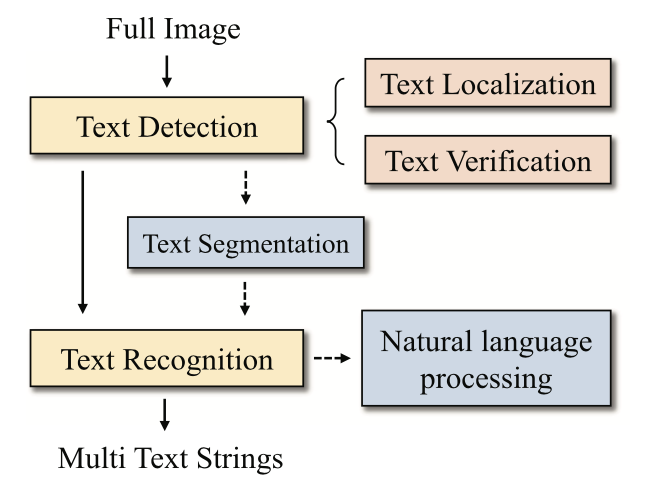
\includegraphics{img/OCR-Basics.png}


\textbf{no source}
grid: divides image into parts $\rightarrow$ each part has own bounding boxes
bounding boxes:~regressor for box, each bounding box is assigned an anchor box (respective to grid cell)
anchor boxes:~default `shape' for bounding box

bounding boxes different stages of convolution / 2-d size $\rightarrow$ different object size to detect

\subsection*{Text detection}
subfield of object detection (e.g. YOLOv4 can be used for text)

Detect position coordinates containing text in input image
Text detection more challenging

Two object detection methods --- CNN-based
\begin{itemize}
    \item Region-based \\
        views detection problem as classification problem\\
        CNN to extract deep features of proposals by selective search $\rightarrow$  Use SVM to
            classify with features\\
        e.g. R-CNN
    \item  single `look'
        extract feature maps on entire image\\
        directly regress bounding boxes on feature maps\\
        e.g. YOLO --- You Only Look Once, SSD --- Single Shot Detection
\end{itemize}
Non CNN-based: DETR

\subsubsection*{Comparison Object Detection basic algos}
\textbf{Comparative analysis of deep learning image detection
algorithms}~\citep{srivastava_comparative_2021}
YOLO-V3 outperforms SSD and Faster R-CNN

VGG-16 widely used feature generating architecture

\subsubsection*{Faster-RCNN}
A deeper look at how Faster-RCNN works~\citep{goswami_deeper_2018}
composed of 3 neural nets:
\begin{itemize}
    \item Feature Network: pre-trained image classification netork $\rightarrow$ generate good features
    \item Region Proposal Network:
        \begin{itemize}
            \item NN with 3 conv layers
            \item one layer splits up network to: classification and bounding box regression
            \item bounding box regression $\rightarrow$ bounding boxes are region of interes (ROI)
                that might contain an object
        \end{itemize}
    \item Detection Network: take input from previous nets, generate final class and bounding box,
        4 fully connected, 2 stacked common layers shared by classification and bounding box regression
        layer \end{itemize}

\textbf{Deep Learning in Character Recognition Considering Pattern Invariance
Constraints}~\citep{oyedotun_deep_2015}
Neural networks can learn features of task on which they are designed and trained
Neural networks better than other approaches (e.g.\ template matching, syntactic analysis)
$\rightarrow$ NNs can learn and adapt to moderate variations (e.g.\ translation, rotation, scaling,
noisy patterns)

\subsection*{Text Recognition}
Recognize text based on position coordinates

character based or word based

Visual attention models for scene text recognition~\citep{ghosh_visual_2017}
Divided into word detection (generate bounding boxes) and word recognition
word recognition can be divided into dictionary-based methods and unconstrained methods

\subsection*{End-To-End}

\chapter{Current Research}\label{ch:research}
no transformers $\rightarrow$ self-attention mechanism is too computationally expensive???

model-pruning $\rightarrow$ remove connections for better performance
\section{Selection}


\section{Review}
`The great advances that have been made in fields such as computer vision and speech recognition,
have been accom- plished by replacing a modular processing pipeline with large neural networks
that are trained end-to-end [37]. In essence, transparency is traded for accuracy.
This is an unavoidable reality.'\citep{arpteg_software_2018}

include Pipeline differences

% FIXME: approaches to research: Faster R-CNN, Mask R-CNN, Yolo v3
% FIXME: look at Backbones: DETR-DC5-R101 and Faster RCNN-R101-FPN+

Two models that can be used in conjunction
\textbf{detection}~\citep{beom_text_2021}\\
uses RetinaNet structure~\citep{lin_focal_2018}\\
applies techniques from textboxes++~\citep{liao_textboxes_2018}

\textbf{character recognition}~\citep{beom_crnn_2021}\\
needs cropped text area as input\\
uses CRNN~\citep{shi_end--end_2015} $\rightarrow$ end-to-end learning, LSTM fir arbitrary length of
input and output, no need to apply detection and cropping to each single character

Open Source OCR engine~\citep{smith_overview_2007}
\begin{itemize}
    \item uses Deep Learning (found c++ code for layers in repo)
    \item Processing in step-by-step pipeline, some unusual stages\\
        1. Line and Word finding\\
        1.1. Line finding\\
        1.2. Baseline Fitting\\
        1.3. Fixed Pitch Detection and Chopping\\
        1.4. Proportional Word Finding\\
        2. Word Recognition\\
        2.1 Chopping Joined Characters\\
        2.2 Accociating Broken Characters\\
        3. Static Character Classifier\\
        3.1 Features\\
        3.2 Classification\\
        3.3 Training Data\\
        4. Linguistic Analysis\\
        5. Adaptive Classifier
\end{itemize}
Performs poorly with unstructured text with significant noise

An Efficient and Accurate Scene Text Detector~\citep{zhou_east_2017}

SOFT:\ Softmax-free Transformer with Linear Complexity~\citep{lu_soft_2021}

Generative Pretraining from Pixels~\citep{chen_generative_2021}
\begin{itemize}
    \item unsupervised representation learning (approach transfered from NLP)
    \item training of sequence Transformer to auto-regressively predict pixels without incorporating
        knowledge of 2D input structure
    \item Active part: GPT-2 scale model learns image representations and performs extremely well even
        when compared to supervised models
\end{itemize}

Learning High-Precision Bounding Box for Rotated Object Detection via Kullback-Leibler
Divergence~\citep{yang_learning_2021}
\begin{itemize}
    \item Deductive approach to rotated object detection
    \item box is `translated' to 2D-Gaussian $\rightarrow$ KLD with prediction and true gaussian as Loss
    \item LIMIT:\ cannot be directly applied to quadrilateral detection
\end{itemize}

DP-SSL:\ Towards Robust Semi-supervised Learning with A Few Labeled Samples~\citep{xu_dp-ssl_2021}
\begin{itemize}
    \item Semi-supervised learning:
        \begin{itemize}
            \item provides way to leverage unlabeled data by pseudo labels
            \item performs poorly and unstable when size of labeled data is very small (low quality
                of pseudo labels)
        \end{itemize}
    \item Data programming:
        \begin{itemize}
            \item paradigm for the programmatic creation of training sets
            \item existing methods rely on human experts to provide initial labeling functions (LF)
        \end{itemize}
    \item DP-SSL
        \begin{itemize}
            \item multiple-choice learning (MCL) based approach to automatically generate labeling functions
            \item scheme to generate probabilistic labels for unlabeled data
        \end{itemize}
\end{itemize}

which aspects to compare? quantitative, qualitative

\chapter{Discussion}\label{ch:discussion}
\section{Analysis}
Plan
\begin{itemize}
    \item Go down hierarchy and compare most important advances
\end{itemize}

For comparison: which Benchmark Dataset fits the problem the best?
\begin{itemize}
    \item~\cite{liao_mask_2020}:
        \begin{itemize}
            \item Rotated ICDAR 2013 (changed normal icdar): rotation robustness
            \item Total-Text: shape ropustness
            \item MSRA-TD500: aspect ratio ropustness
        \end{itemize}
    \item~\cite{yang_learning_2021}:commonly used for oriented text: ICDAR2015, ICDAR2017 MLT, MSRA-TD500
\end{itemize}

Important points:
\begin{itemize}
    \item ResNet is pretty much the Feature Extractor Benchmark
\end{itemize}

Recognition
\begin{itemize}
    \item Ability to cope with 2d text:
        CTC has problems,
        Attention/Encoder-Decoder based can be extended to work
    \item CTC prone to overfitting
    \item Attention has problems with long sequences
\end{itemize}

\section{Reflection}
Threats to validity!
\begin{itemize}
    \item~\cite{arpteg_software_2018}: different papers have different components
        $\rightarrow$ Hardware, Platform, Source Code, Configuration
        $\rightarrow$ studies can't really be compared
    \item~\cite{arpteg_software_2018}: `A major challenge in developing DL systems is the
        difficulties in estimating the results before a system has been trained and tested.'
    \item~\cite{long_scene_2021}: different interpretations of metrics (matching for \ac{STD},
        word/char for \ac{STR})
    \item~\cite{siebert_construction_2021,nakamichi_requirements-driven_2020}: all entities of
        \ac{MLS} should be inspected when developing a solution
    \item~\cite{baek_what_2019}: different papers use different evaluation and testing environments
    \item~\cite{baek_what_2019}: different papers use different subsets of the same dataset
        $\rightarrow$ discrepancies in performance
    \item~\cite{long_unrealtext_2020}: half of the widely adopted benchmark datasets have imperfect
        annotations $\rightarrow$ ignoring case-sensitivities and punctuations, and provide new
        annotations for those datasets
    \item~\cite{chen_text_2021}: inconsistency of datasets, priors and testing environments make
        comparison difficult
\end{itemize}

\section{Outlook}

\begin{itemize}
    \item next steps to practically solve problem $\rightarrow$  Data Collection, Data Cleaning,
        Data Labeling, Model Training, Model Evaluation, Model Deployment, Model
        Monitoring~\citep{watanabe_preliminary_2019}
    \item  Use Neural Architecture Search to automatically find right feature
        extractor~\citep{zhao_improving_2020}
    \item~\cite{siebert_construction_2021,nakamichi_requirements-driven_2020}: build system around
        model $\rightarrow$ e.g.\ supervision mechanism
    \item~\cite{shi_icdar2017_2017,he_icpr2018_2018}: adjust field to better metrics for evaluation
    \item~\cite{long_scene_2021}: general trend to move towards simpler,shorter pipeline
\end{itemize}

\chapter{Conclusion}
This thesis provides a comprehensive overview of techniques that are used for \ac{STS}.
The associated tasks and the different approaches help compare different
solutions for the identified qualified that are important for the use case
(appropriateness, performance/robustness, efficiency).

The overview and literature review reveal that \ac{STD} and \ac{STR} are concerned
with robust performance for multi-oriented and curved text instances.
For \ac{STD}, the more efficient \ac{BB} regression-based methods can detect multi-oriented text well.
Because of \acp{BB}' representational deficiencies, pixel-level segmentation-based methods are better for
detecting curved text.
However, they are more computationally expensive.
For the semantics retention subquality for appropriateness, it is, therefore, essential to consider
the text properties of the dataset.
The attention mechanism has become the primary approach for \ac{STR} robustness.
However, many innovations are concerned with the curved text rectification stage that both
\ac{CTC} and attention-based \ac{EnDe} solutions share.
\ac{CTC} has the advantage over the attention mechanism for recognition of alphanumeric strings
and efficiency, while attention is better with recognizing curved text.
For \ac{STS} research, 2-stage approaches are the focus because of their remarkable efficiency and
competitive performance.
The efficient combination of \ac{STD} and \ac{STR} stages and reuse of feature maps are topics
of the innovations in the field.

For future work, it would be helpful to consider different steps in the \ac{ML}
lifecycle~\citep{watanabe_preliminary_2019} or build a \ac{MLS} around the identified \ac{DL}
approach for \ac{STS}~\citep{siebert_construction_2021,nakamichi_requirements-driven_2020}.
An example would be to design a supervision mechanism for model monitoring that is important for
\ac{DL} in production systems~\cite{nakamichi_requirements-driven_2020,watanabe_preliminary_2019}.
Another possible step would be to design and carry out a comprehensive study to generate quantitative
data regarding the qualities that a \ac{STS} solution must possess.


\appendix

\chapter{References}

% Literaturverzeichnis
%\bibliographystyle{dbstmpl}    % verwendet dbstmpl.bst
\bibliographystyle{alpha}

% alternative, vorinstallierte Stile sind z.B. plain oder abbrv
\bibliography{dbstmpl}         % verwendet dbstmpl.bib

\chapter{Code}
\end{document}
